\documentclass[reqno, 12pt]{amsart}
\usepackage{amsmath,amssymb,amsthm}
\usepackage{xcolor}
\usepackage{tikz}
\usepackage[T1]{fontenc}

\begin{document}

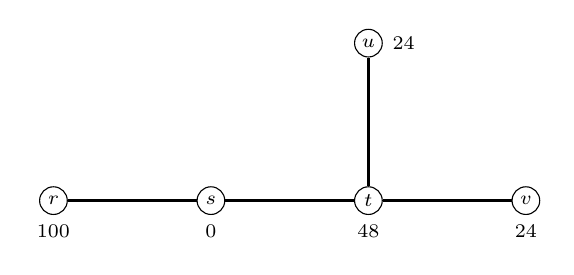
\begin{tikzpicture}
    [scale=2.0]
    \tikzset{vertex/.style = {circle, draw=black, fill=white!100, inner sep=0pt, minimum width=10pt}}
    \tikzset{vertex1/.style = {circle, draw, fill=white!100, inner sep=0pt, minimum width=10pt}}
    \tikzset{edge0/.style = {line width=1pt, black}}

    \node [vertex, label=below:{$\scriptstyle{100}$}] (v0) at (1,0) {$\scriptstyle{r}$};
    \node [vertex, label=below:$\scriptstyle{0}$] (v1) at (2,0) {$\scriptstyle{s}$};
    \node [vertex, label=below:$\scriptstyle{48}$] (v2) at (3,0) {$\scriptstyle{t}$};
    \node [vertex1, label=below:$\scriptstyle{24}$] (v3) at (4,0) {$\scriptstyle{v}$};
    \node [vertex, label=right:$\scriptstyle{24}$] (v4) at (3,1) {$\scriptstyle{u}$};

    \draw[edge0] (v0) -- (v1);
    \draw [edge0] (v1) -- (v2);
    \draw [edge0] (v2) -- (v3);
    \draw[edge0] (v2) -- (v4);
\end{tikzpicture}

\end{document}